\section{Design}
\label{sec:design}

Networked systems as used today consist of many hardware and software components that are connected to each other to achieve their intended task.
Hosts in a network use gateways to communicate with hosts in other networks, user space applications use system calls to interact with the operating system and hardware components use interfaces to achieve interaction between each other, such as PCI.
However, many of the components can not be updated or upgraded, either due to their proprietary nature or due to lengthy standardization and deployment processes.
This hinders the development of novel applications or improvements of existing systems.
However, developers and engineers already found a way to overcome this problem, by utilizing the environment of such systems and force it behave as desired.

\subsection{Unobtrusive Mechanism Migration by Example}
To illustrate this idea, two examples will be given.

\subsubsection{Network Address Translation}
The Internet Protocol version 4 (IPv4) was designed in the late 1970s and deployed throughout the 1980s.
At that time, the number of participating hosts in the Internet was rather low with less than 1000 and the designers of IPv4 did not anticipate, that the number of hosts in the Internet would increase dramatically as it did especially since the 2000s.
Thus, they chose a 32 Bit field for addressing, allowing only roughly 4.3 billion hosts in the Internet.
With over 5.5 billion devices~\cite{eriscsson2021report}, there are even more smartphones already available globally, not to mention servers, wearables, embedded systems and the entire IoT area.
This development raised the need for solutions.
Althouth there is a newer version of the IP, IPv6 allowing $2^128$ ho

Das erste Beispiel: NAT
Problem, das NAT lösen soll: IPv4 Adressen gibt es zu wenige. Das Ausrollen neuer, besseren Standards dauern jedoch lange, müssen parallel betrieben werden
Sytem: Host, der über das Internet kommunizieren möchte
Environment: Netzwerkzugang
Interceptor: Softwarekomponente auf dem Gateway, der das masquerading anbietet.
Alter mechansimus: routing auf dem Gateway
Neuer Mechanismus: routing wird druch hinzugefügtes masquerading ersetzt
Hinweis: dieses beispiel sollte etwas ausführlicher dargestellt werden, also was wird konkret intercepted, wie findet die Übersetzung statt.

\paragraph{Example 2: WINE}
Zweites Beispiel: Wine
Problem: Ausführung von Programmen auf Betriebssystemen mit inkompatiblen Schnittstellen und Bibliotheken; eine spezifische Implementierung in eimem Anderen Betriebssytem würde das Problem nur für das spezifische System lösen, wine löst es generell durch das Interceptor patter.
System: Programm
Environment: Betriebssytem
Interceptor: Sammlung an überschriebenen Sytemaufrufen und Bibliotheken, Wine
Alter mechanismus: Nutzung der vom betriebyssytem bereitgestellten systemafurufe und bibliotheken
neue Mechanismus: Nutzung von POSIX schnittstellen über hinzugefügte systemafurufe und bibliotheken
Hinweis: auch dieses Beispiel ausführlicher Beschreiben

Die Informatik ist voll von solchen Abstraktionen, etwas <hier zwei weitere Beispiele einsetzen>.
Das ist nicht nur eine Anomalie oder Ausnahme von Funktionserweiterung.
Wie posulieren, dass dieses Vorhegen System hat, sodass wir eine Abstraktion definieren.


\subsection{System Model}
\begin{figure}
    \centering
    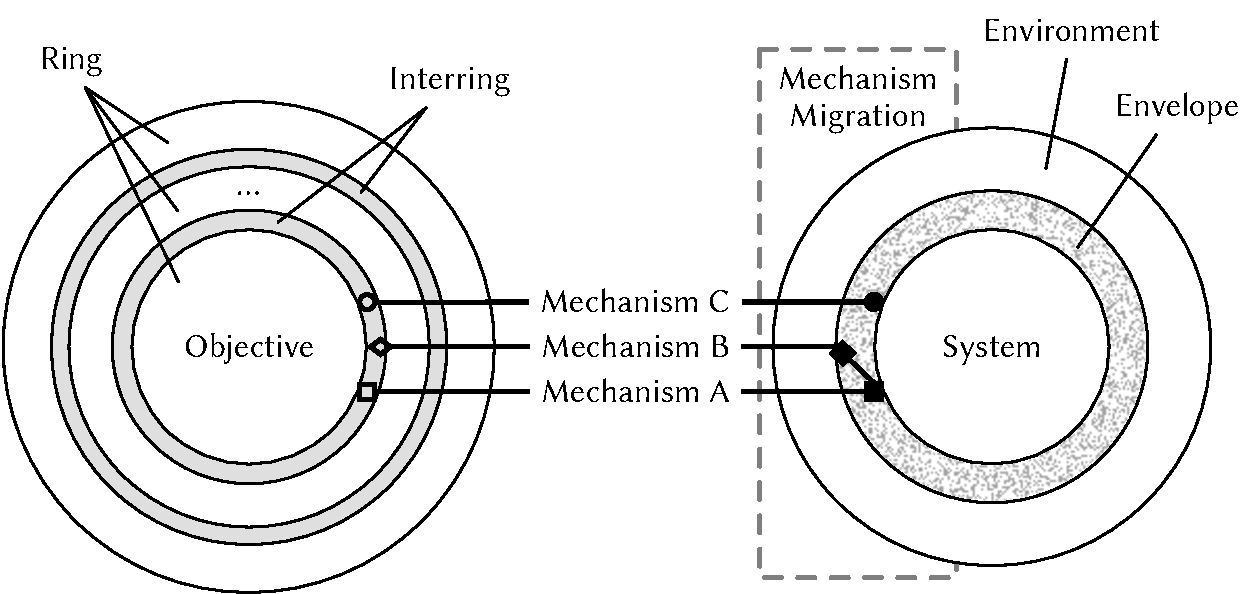
\includegraphics[width=\linewidth]{figures/MechanismMigration.pdf}
    \caption{Mechanism migration to a legacy device with transition-enabled environment}
    \label{fig:bigpicture}
\end{figure}

% Das von uns abgeleitete Modell besteht aus folgenden Komponenten:
The model derived from the above examples and further observations consists of the following components:


\paragraph{System}
At the core of the consideration lies a system that is intended to achieve a specific task.
The system cannot be changed because it is a proprietary component or depends on other external factors, such as high coordination costs for changes due to long standardization or technical hurdles.
This is necessarily so that the system can fulfill its actual task. 
For example, the host in the NAT example needs the routing functionality of the gateway to enable communication with hosts in other networks.

\paragraph{Environment}
Every system is surrounded by an environment that provides functionality for use.
The system has a dependency relationship with the environment, as the system is dependent on the functions provided.
This is necessarily so that the system can fulfill its actual task. For example, the host in the NAT example needs the routing functionality of the gateway to enable communication with hosts in other networks.

\paragraph{Mechanism}
By a mechanism, we refer to the concrete implementation of a functional unit of the environment that is used by the system to achieve its task.
% By a mechanism, we refer to ''a confined conceptual element of a (networked) system that is bound to a realization as cooperating functional units''~\cite{frommgen2016mechanism}.
Mechanisms are located at various points of hardware/software systems, for example:

\begin{itemize}
 \item Complete protocols: TCP, UDP, RTP, overlays, etc.
 \item Specific parts of protocols: congestion control, fragmentation, load balancing, replication, etc.
 \item Network concepts: infrastructure-based, ad-hoc, partially meshed, delay tolerant (DTN), etc.
 \item Network technologies: Ethernet, LTE, IEEE 802.11, Bluetooth, etc.
 \item Security mechanisms: encryption, integrity protection, authentication, etc.
 \item System components: positioning (via WLAN, GSM or GPS), sensors, etc.
 \item Operating System APIs
 \item System Bus Interfaces
\end{itemize}



\paragraph{Interceptor}
In the field of software development, the ``Interceptor architectural pattern allows services to be added transparently to a framework and triggered automatically when certain events occur''~\cite{schmidt2013pattern}.
In this programming pattern, a framework provides interfaces so that programs using this framework can transparently intervene in the flow of data at specific events.

While the goal of our interceptor is basically the same, namely to transparently intervene in the data flow and thus enable new functionalities, the perspective is reversed.
An interceptor in our definition is part of the environment and provides mechanisms to the system via known interfaces. 
In contrast to the interceptor pattern of software engineering, the interceptor is used by the system but configured by the environment so that its use is inevitable.
In order for the system to use the new mechanism, the interceptor is inserted between the system and the mechanism and changes the data flow.
The mechanism to be used can also be introduced into the environment as part of the interceptor and does not have to exist a priori. 


\paragraph{Unobtrusive}
In order not to influence or even disturb the actual task of the system, the mechanism from the interceptor must be unobtrusively replaced by the provided mechanism.
The system must not notice the change of the mechanism, on the contrary the used interfaces must suggest that the original mechanism would be in force.
Furthermore, an interceptor must be unobtrusive so that the system can continue to fulfill the functionality and not provide error cases for the termination.




































%%%%%%%% OLD %%%%%%%%%%%%%
% \begin{figure}
%     \centering
%     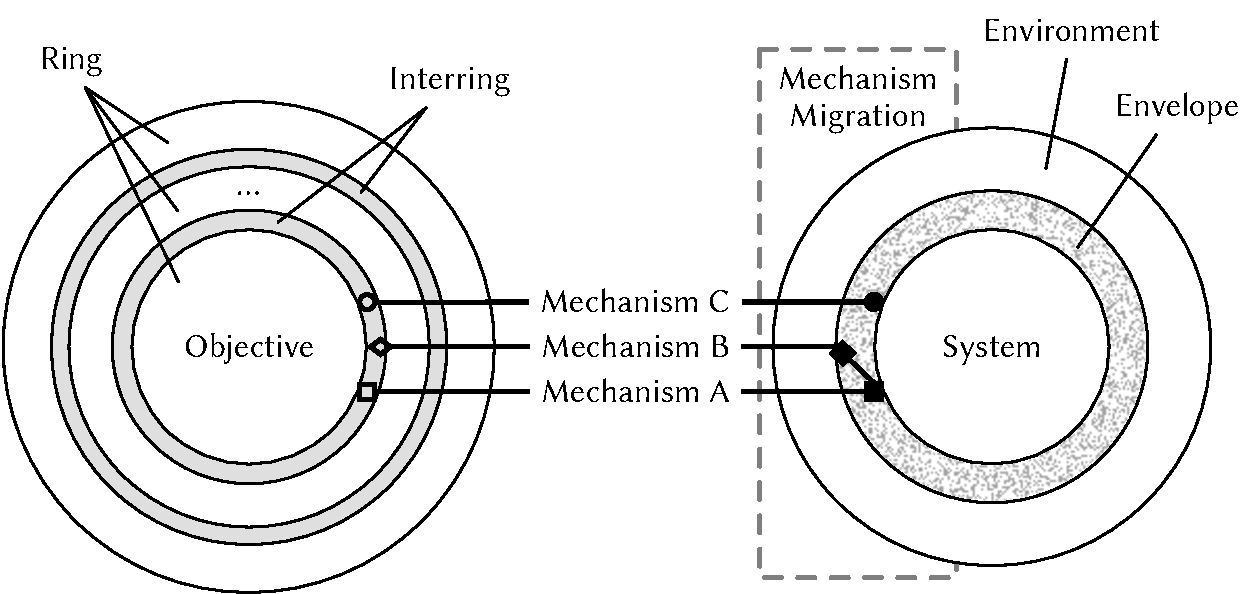
\includegraphics[width=\linewidth]{figures/MechanismMigration.pdf}
%     \caption{Mechanism migration to a legacy device with transition-enabled environment}
%     \label{fig:bigpicture}
% \end{figure}

% The concept of \emph{\mm} allows altering behavior of information and communications system (ICS) that are incapable or unwilling to modify their own operation.
% This could be due to an ICS being built upon proprietary frameworks disallowing modification of the device, manufacturers dropping support or by the unwillingness to make the effort to adapt or update the components of the ICS.
% In such cases developers or network operators are unable to modify the ICS itself.
% However, the proposed approach of \mm enables the modification of an ICS's environment to enforce the desired adaption in its behavior.
% This change can be thought of as an ''outer'' level of the communication infrastructure enveloping an ''inner'' level.

% For example, when faced with a closed application executed on a smartphone, operating system (OS) might be modified to force the applications behavior to change by modifying the OS network stack to transparently wrap connection in a VPN.
% If a whole device is unmodifiable, but the network is under control of the network operator the network can be utilized to force the device to behave in a desired way, e.g. by placing gateway-servers inside the network who can transparently alter traffic flows.
% If even the network is outside control modifying or replacing the communication partner/backend with which the device is communicating is possible.


% \subsection{Rings}
% As the above examples suggest, modern information and communications technology consists of a multitude of components like access devices (smartphones, computers, etc.) and network infrastructure (routers, back-bone network), software (e.g., OSs, middle-ware, applications), networks, network topologies, network protocols on various layers, compute facilities (cloud, edge, etc.) and so on.
% We subdivide these components into a ring structure, as shown in \Cref{fig:bigpicture}, where each \emph{ring} represents a component required for the given domain.
% The most specific component, whose functionality is to be improved by the proposed \mm, forms the center of the structure, called \emph{objective}, while other components are added as rings.
% As an example, an ICS providing a VoIP service to users, the telephony application installed on the end-users device would form the objective, as it should be modified in some way.
% This application requires the OS and its networking APIs, which forms the ring around the application, whereas the next outer ring forms the local area network.
% This categorization allows arbitrary deep rings that seem appropriate for the given domain.
% In the above example, the outer most ring would be the backend executed on a server in the cloud.
% For enabling \mm, it is important to be able to modify or alter rings around the objective, although it is not required to have control of all rings but only the ring required to achieve the desired result.


% \subsection{Interrings}
% Between adjacent rings, components require interaction.
% Such an interface can be anything from set of rules governing the actual communication, such as protocols defined on the different layers of the network-stack-model, to implicit assumptions over the inner workings of peers in a network.
% In the above example, the telephony application uses the OS's networking API to send and receive data.
% Thereon, the OS uses for example Wi-Fi or cellular connectivity to access the local area network, and so on.
% These interaction layers are called \emph{interrings} and are represented as gray layers between the rings in \Cref{fig:bigpicture}.
% Beyond the network stack on a local device itself, interrings include any functionality that allows interaction between two rings like system calls in an application-OS relation or communications between multiple nodes in a network.


% \subsection{Mechanism}
% A \emph{mechanism} is a functional part of an interring that realizes functional units to achieve the desired functionality of the objective.
% Examples of such mechanisms are manifold and span all protocol- and system-layers, as the following selection of possible mechanisms shows:

% \begin{itemize}
%  \item Complete protocols: TCP, UDP, RTP, overlays, etc.
%  \item Specific parts of protocols: congestion control, fragmentation, load balancing, replication, etc.
%  \item Network concepts: infrastructure-based, ad-hoc, partially meshed, delay tolerant (DTN), etc.
%  \item Network technologies: Ethernet, LTE, IEEE 802.11, Bluetooth, etc.
%  \item Security mechanisms: encryption, integrity protection, authentication, etc.
%  \item System components: positioning (via WLAN, GSM or GPS), sensors, etc.
% \end{itemize}

 

% \subsection{Envelope, System and Environment}
% In order to realize the proposed approach, it is necessary to migrate novel functionality to existing ICS.
% An \emph{\env} is a component containing such a new or alternative mechanism that is migrated to the interring between the last ring that is under control and the first ring that is not under control.
% For example, if the telephony application that should support vertical handovers is not modifiable but the OS, the \env containing a mechanism enabling vertical handovers could be placed in the interring between application and the OS.
% It might also be desirable to migrate an \env into an outer interring, although a ring closer to the objective might be still under control.
% All rings, including the objective, that are located within the \env are summarized as the \emph{system} and all rings outside the \env are called \emph{environment}.

 